\subsection{Cбор данных}
\label{sec:experiment:data_loading}

В связи с тем, что рынок вторичного жилья лучше соответствует рыночным принципам формирования цен на основе спроса и
предложения, в отличие от цен, устанавливаемых компанией-застройщиком жилья на первичном рынке, определение рыночной
стоимости, как наиболее вероятной цены продажи объекта недвижимости, более целесообразно провести на примере объектов
недвижимости вторичного рынка жилья. При создании модели оценки жилой недвижимости в качестве входных параметров были
включены факторы, представленные в таблице~\ref{table:experiment:data_loading:data_model}:

\begin{table}[!ht]
\caption{Характеристики недвижимости}
\label{table:experiment:data_loading:data_model}
\centering
	\begin{tabular}{{ 
	|>{\centering}m{0.2\textwidth} | 
	 >{\raggedright\arraybackslash}m{0.74\textwidth}|}}

  	\hline
  	Параметр & {\begin{center} Описание \end{center}} \\

    \hline
    Price & Стоимость данного объекта\\

    \hline
    District & Район города\\
    
    \hline
    Rooms count & Количество комнат\\

    \hline
    Floor & Этаж\\

    \hline
    House Type & Тип дома(панельный, монолитный, кирпичный, каркасно-блочный)\\

    \hline
    Area full & Полная площадь, кв.м\\

    \hline
    Area living & Жилая площадь, кв.5\\

    \hline
    Build year & Год постройки дома\\

    \hline
    Bathroom type & Тип санузла(раздельный, совмещенный)\\

    \hline
    Finishing & Ремонт(хороший, плохой, без отделки, и т.д.)\\

  \hline
  \end{tabular}
\end{table}

Исходные данные были взяты из базы проданной недвижимости в г. Минске на момент конца 2020 года.
Данные собраны с сайта realt.by с помощью технологии веб-скрапинга. Это технология получения данных путем извлечения
их со страниц веб-ресурсов. Для скрапинга использовался язык программирования Ruby. Данный язык удобен тем, что
поддерживает множество сторонних библиотек, помогающих в сборе данных.
Всего было собрано данных о более чем 8 тысяч продающихся объектов недвижимости, которые затем были
экспортированы в формате csv.
Данные хранятся в виде таблицы, часть которой показана на рисунке~\ref{fig:experiment:csv_example}

\begin{sidewaysfigure}
  \centering
    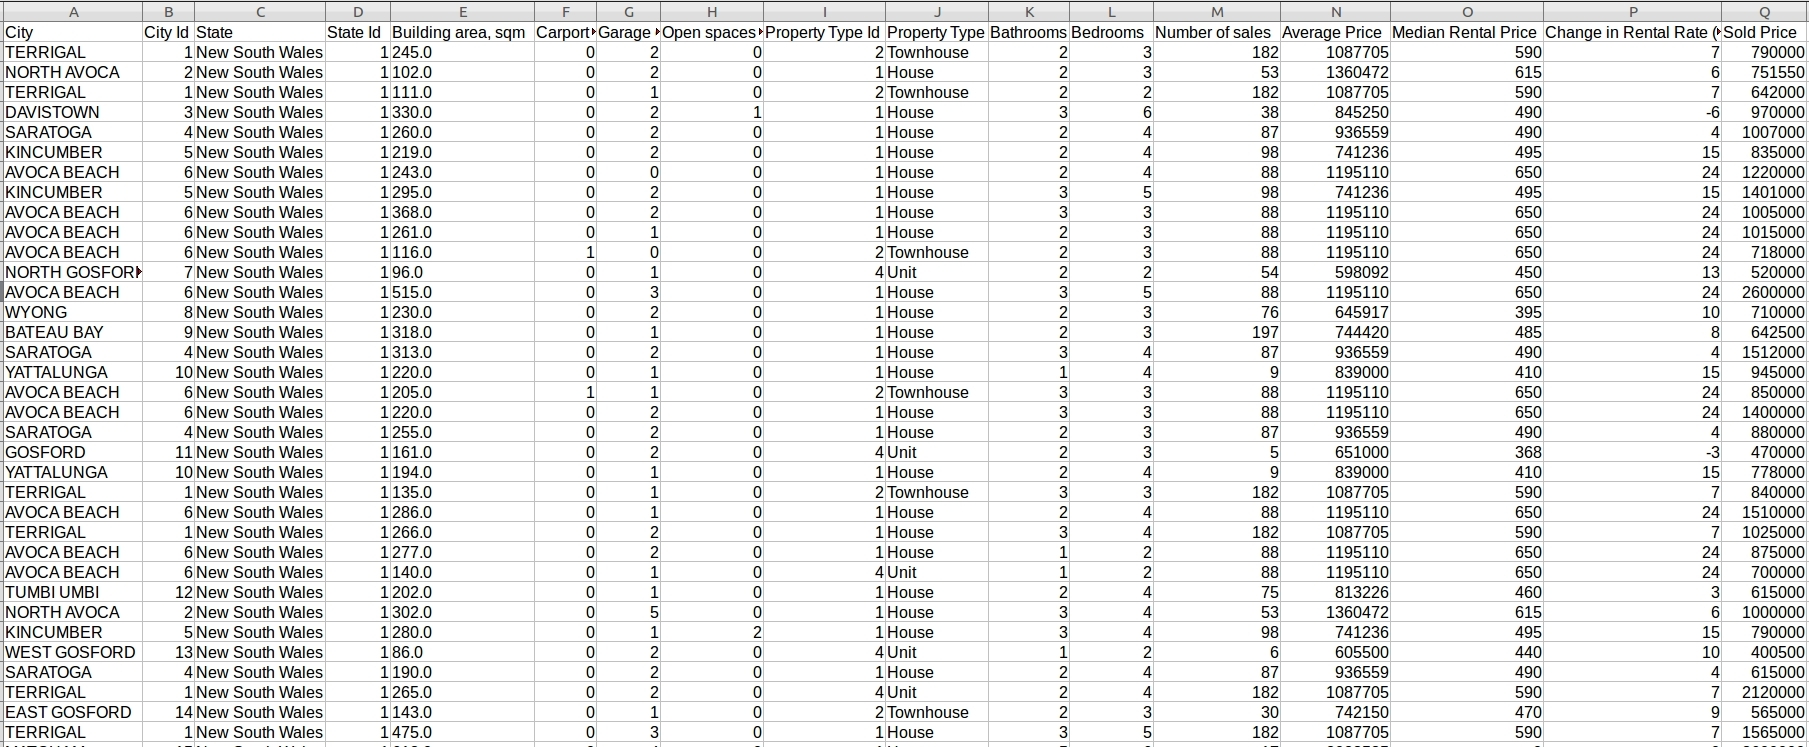
\includegraphics[scale=0.5]{csv.jpg}
    \caption{Исходные данные в csv формате}
    \label{fig:experiment:csv_example}
\end{sidewaysfigure}
